
%(BEGIN_QUESTION)
% Copyright 2010, Tony R. Kuphaldt, released under the Creative Commons Attribution License (v 1.0)
% This means you may do almost anything with this work of mine, so long as you give me proper credit

Show how to connect the loop calibrator to measure the pressure transmitter's current signal, with the calibrator set in ``measure'' (read) mode to act like a milliammeter:

$$\includegraphics[width=15.5cm]{i04727x01.eps}$$

\underbar{file i04727}
%(END_QUESTION)





%(BEGIN_ANSWER)

Award half credit for proper connection point (anywhere in {\it series} with the transmitter circuit) and half credit for proper polarity (conventional flow entering the calibrator's red lead and exiting the black lead).

%(END_ANSWER)





%(BEGIN_NOTES)

{\bf This question is intended for exams only and not worksheets!}

%(END_NOTES)


